\documentclass[float=false, crop=false]{standalone}
\linespread{1.3}

\usepackage[subpreambles=true]{standalone}
\usepackage{import}

\usepackage{parskip}
\setlength{\parindent}{0pt} %no paragraph indentation
\setlength{\parskip}{2.1ex plus 0.2ex minus 0.2ex} %3x paragraph spacing

\usepackage{geometry}
\geometry{letterpaper,left=1.0in,right=1.0in,top=1.0in,bottom=1.0in}

\usepackage{fancyhdr}
\pagestyle{fancy}
\fancyhf{}
\renewcommand{\headrulewidth}{0pt}
\rfoot{\thepage}

\usepackage{hyperref}

\usepackage[fleqn]{amsmath}
\usepackage{amssymb}
\usepackage{amsthm}

\usepackage{graphicx}
\graphicspath{{./imgs/}}

\begin{document}
	
	In \cite{Kambam2008} the authors design a synthetic consortium between two strains of E. coli using a quorum-sensing mechanism. The engineered genetic circuits added to each strain are shown in figure~\ref{fig:kambam2008_genecircuits}.
	\begin{figure}[h]
		\centering
		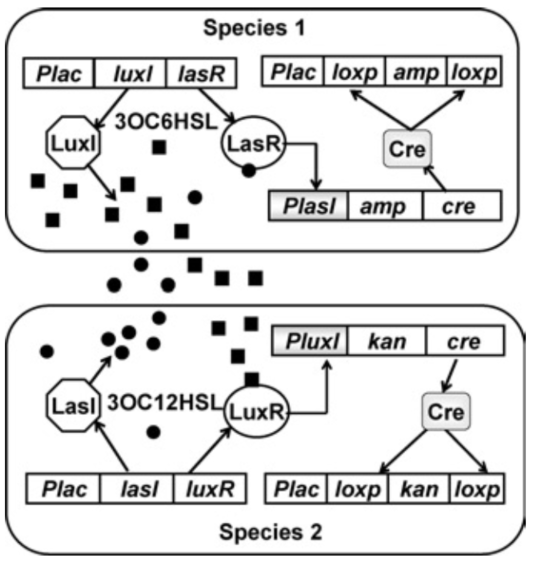
\includegraphics[width=0.5\textwidth]{kambam2008_genecircuits.png}
		\caption{E. coli gene circuits.}
		\label{fig:kambam2008_genecircuits}
	\end{figure}
	Each species constitutively expresses the \textit{amp} and \textit{kan} genes which code for resistance to the antibiotics ampicillin and kanamycin respectively. However, the constitutively expressed resistance gene located between the \textit{loxp} genes can be removed by expression of the \textit{cre} gene. This gene is regulated by the transcription factor \textit{LasR} and \textit{LuxR} in each species respectively. The quorum-sensing modules \textit{LuxI}/\textit{LuxR} and \textit{LasI}/\textit{LasR} are also used to promote expression of the resistance gene located on a different circuit. When the cell densities reach some critical level the \textit{Cre} enzyme knocks out the constitutively expressed resistance gene. Thus expression of the resistance gene in each species is regulated by the expression of AHL in the complementary microbe.  
	
	A model of this system was used to infer sensitivity and importance of parameters. While the authors did not actually implement their design the mathematical model they developed allowed them to understand the most important variables governing mutualism for their system. For example, the growth rate of species 2 is significantly higher than species 1. Without the designed interactivity species 1 would rapidly become extinct due to inter-species competition. By incorporating obligatory mutualism in the system, and manipulating the pertinent parameters identified by the model, the authors found that it is possible to vary the steady state cell density ratio.    
	  	
	\ifstandalone
		\bibliographystyle{unsrt}	
		\bibliography{../../../Research/library}
	\fi

\end{document}